% ch6.tex
% This work is licensed under the Creative Commons Attribution-Noncommercial-Share Alike 3.0 New Zealand License.
% To view a copy of this license, visit http://creativecommons.org/licenses/by-nc-sa/3.0/nz
% or send a letter to Creative Commons, 171 Second Street, Suite 300, San Francisco, California, 94105, USA.


\chapter{Sort of like recycling$\ldots$}\label{ch:sortoflikerecycling}

Think about how much rubbish you create each day. Bottled water or bottles of soft drink, packets of crisps, plastic sandwich wrappers, bags of vegetables, meat on plastic trays, plastic shopping bags, newspapers, magazines, and so on and so on and so on$\ldots$
\par
Now just think about what would happen if all of that trash just got dumped in a pile at the end of your driveway.

\begin{center}
\includegraphics*[width=100mm]{eps/trash.eps}
\end{center}

Of course, you probably recycle as much as possible.  Which is fortunate, because no one likes having to climb over a rubbish heap, on the way to school.  So, those glass bottles in the recycle bin are hopefully melted down, and then turned into new jars and bottles; paper is pulped into recycled paper; plastic turned into heavier plastic goods---so your front lawn doesn't disappear under tonnes of garbage. We get to reuse some of the goods we create, rather than eating a gaping hole in the side of the world to manufacture the same things over and over again.

Recycling or reuse, in the programming world, is just as important. Not because your program will disappear under a pile of garbage---but if you don't re-use some of what you're doing, you'll eventually wear your fingers down to painful stubs through over-typing.

There are a number of different ways to reuse code in Python (and in programming languages in general), but we've seen one of the ways already, back in Chapter 3, with the function range.  Functions\index{functions} are one way to reuse code---so you can write the code once, then use it in your programs again and again.  Let's first try a simple example of a function:

\begin{listing}
\begin{verbatim}
>>> def myfunction(myname):
...     print('hello %s' % myname)
...
\end{verbatim}
\end{listing}

The above function has a name `myfunction' and has a parameter `myname'.  A \emph{parameter} is a variable which is only available within the `body' of the function (which is the block of code immediately after the line starting with \code{def}---in case you're wondering, \code{def} is short for define).  You can run the function by calling its name with brackets surrounding the parameter value:

\begin{listing}
\begin{verbatim}
>>> myfunction('Mary')
hello Mary
\end{verbatim}
\end{listing}

\noindent
We could change the function to take 2 parameters:

\begin{listing}
\begin{verbatim}
>>> def myfunction(firstname, lastname):
...     print('Hello %s %s' % (firstname, lastname))
...
\end{verbatim}
\end{listing}

\noindent
And then call it in a similar fashion to the first:

\begin{listing}
\begin{verbatim}
>>> myfunction('Mary', 'Smith')
Hello Mary Smith
\end{verbatim}
\end{listing}

\noindent
Or we could create some variables and call the function with the variables:

\begin{listing}
\begin{verbatim}
>>> fn = 'Joe'
>>> ln = 'Robertson'
>>> myfunction(fn, ln)
Hello Joe Robertson
\end{verbatim}
\end{listing}

\noindent
We can return values from a function using the \code{return}\index{return} statement:

\begin{listing}
\begin{verbatim}
>>> def savings(chores, paper, spending):
...     return chores + paper - spending
...
>>> print(savings(10, 10, 5))
15
\end{verbatim}
\end{listing}

This function takes 3 parameters, and then adds the first two (\code{chores} and \code{paper}) before subtracting the last one (\code{spending}).  The result is then returned---this result can be used as the value of a variable (the same way we set other values to variables):

\begin{listing}
\begin{verbatim}
>>> my_savings = savings(20, 10, 5)
>>> print(my_savings)
25
\end{verbatim}
\end{listing}

\noindent
However, a variable that we use inside the body of a function will not be accessible (usable), when the function has finished:

\begin{listing}
\begin{verbatim}
>>> def variable_test():
...     a = 10
...     b = 20
...     return a * b
...
>>> print(variable_test())
200
>>> print(a)
Traceback (most recent call last):
  File "<stdin>", line 1, in <module>
NameError: name 'a' is not defined
\end{verbatim}
\end{listing} 

In the above example we create a function \code{variable\_test}, which multiplies two variables (\code{a} and \code{b}) and returns the result.  If we call this function using \code{print}, we get the answer: 200.  However if we try to print the contents of \code{a} (or \code{b} for that matter), we get the error message ```a' is not defined''. This is something called `\emph{scope}'\index{scope}, in the world of programming.
\par
Think of a function as a little island floating in the ocean---and it's too far to swim from the island to anywhere else.  Occasionally, a plane flies over and drops bits of paper on the island (those are parameters coming into a function) which the inhabitants then stick together into a message, put the message into a bottle and then toss the bottle into the sea (this is the return value).  What the islanders do on the island, and how many of them it took to make the message, makes no difference to the person picking up the bottle and reading the message inside.  This is probably the easiest way to think about scope---but there is one small problem with that idea.  One of the islanders has a large pair of binoculars and can see all the way to the mainland.  He can see what other people are doing there, and that can affect the message that they're creating:

\begin{listing}
\begin{verbatim}
>>> x = 100
>>> def variable_test2():
...     a = 10
...     b = 20
...     return a * b * x
... 
>>> print(variable_test2())
20000
\end{verbatim}
\end{listing}

So, even though variables \code{a} and \code{b} aren't able to be used outside of the function, the variable \code{x} (which was created outside the function) is usable inside.  Just think about the islander with the binoculars, and hopefully it might help that idea to make a little bit of sense.

\begin{center}
\includegraphics*[width=100mm]{eps/islanders.eps}
\end{center}

The for-loop we created earlier to display savings over a year, could easily be added to a function:

\begin{listing}
\begin{verbatim}
>>> def yearly_savings(chores, paper, spending):
...     savings = 0
...     for week in range(1, 53):
...         savings = savings + chores + paper - spending
...         print('Week %s = %s' % (week, savings))
...
\end{verbatim}
\end{listing}

Try entering that function in the console, and call it with different values for \code{chores}, \code{paper} and \code{spending}:

\begin{listing}
\begin{verbatim}
>>> yearly_savings(10, 10, 5)
Week 1 = 15
Week 2 = 30
Week 3 = 45
Week 4 = 60
Week 5 = 75
Week 6 = 90
Week 7 = 105
Week 8 = 120
Week 9 = 135
Week 10 = 150

(continues on...)

>>> yearly_savings(25, 15, 10)
Week 1 = 30
Week 2 = 60
Week 3 = 90
Week 4 = 120
Week 5 = 150

(continues on...)
\end{verbatim}
\end{listing}

This is a bit more useful than re-typing the for-loop every time you want to try it with a different value. Functions can also be grouped together into something called `modules', which is where Python becomes really useful$\ldots$ as opposed to just mildly useful.
\par
\noindent
\emph{More about modules shortly.}

\section{Bits and Pieces}

When Python is installed on your computer, a whole pile of functions and modules are also installed. Some functions are available by default.  \code{range} is a function we've already seen. \code{file}\index{functions!file} is another function we haven't use yet.

\begin{WINDOWS}

To see how \code{file} is used, open Notepad and type a few words, then save the file onto your C drive, by:

\begin{enumerate}
 \item clicking on the File menu, then Save,
 \item double-click on `My Computer' in the file dialog,
 \item double-click on `Local Drive (C:)',
 \item in the File name box (at the bottom) where it says `*.txt', type `test.txt' 
\end{enumerate}

\begin{figure}
\begin{center}
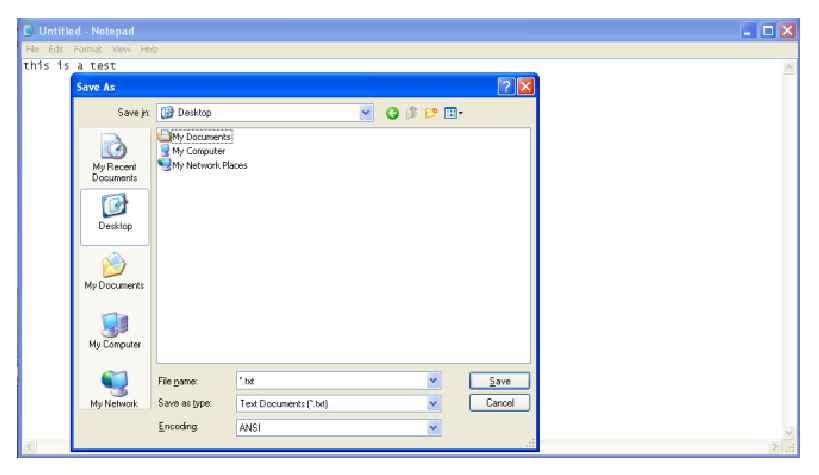
\includegraphics[width=65mm]{eps/figure17.eps}
\end{center}
\caption{The save dialog from Windows Notepad.}\label{fig17}
\end{figure}

Open the Python console again, and try the following:

\begin{listing}
\begin{verbatim}
>>> f = open('c:\\test.txt')
>>> print(f.read())
\end{verbatim}
\end{listing}

The contents of the file you just created should be printed to the console. You can now jump ahead to the bit that says: ``Continuing from here$\ldots$''.
\end{WINDOWS}

\begin{MAC}
To see how \code{file} is used, open up the Text Editor, by clicking on the editor icon (\includegraphics*[width=12mm]{eps/textedit-icon.eps}).  Type a few words then save the file to the Desktop by clicking File, then Save, and entering the name `text.txt' in the entry box next to `Save As'.

\begin{figure}
\begin{center}
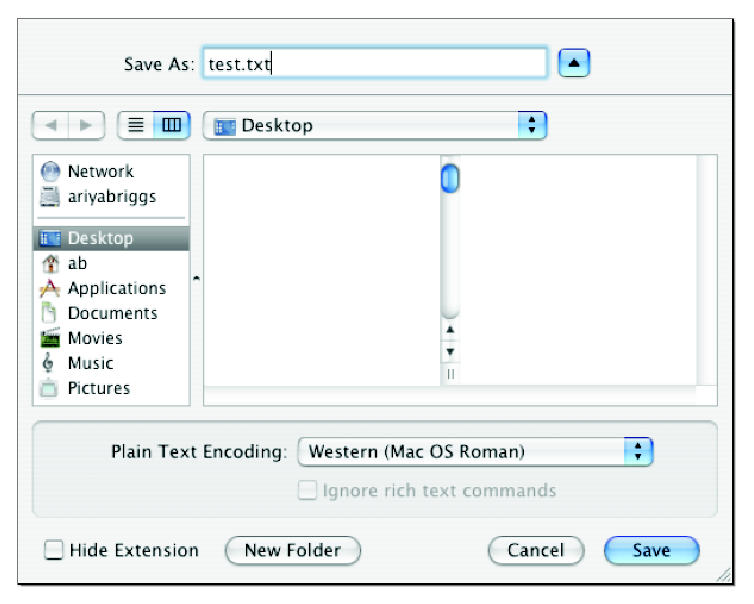
\includegraphics[width=65mm]{eps/figure18.eps}
\end{center}
\caption{The save dialog from Mac OS X Text Editor.}\label{fig18}
\end{figure}

Open the Python console again, and try the following:

\begin{listing}
\begin{verbatim}
>>> f = open('Desktop/test.txt')
>>> print(f.read())
\end{verbatim}
\end{listing}

The contents of the file you just created should be printed to the console.  You can now jump ahead to the bit that says: ``Continuing from here$\ldots$''.
\end{MAC}

\begin{LINUX}
To see how \code{file} is used, open a text editor, type a few words and then save the file to your home directory, by clicking File, Save, selecting `Home Folder' (or `Home Directory' or `Home') and typing `test.txt' in the file name box (see figure~\ref{fig19} for an example).

\begin{figure}
\begin{center}
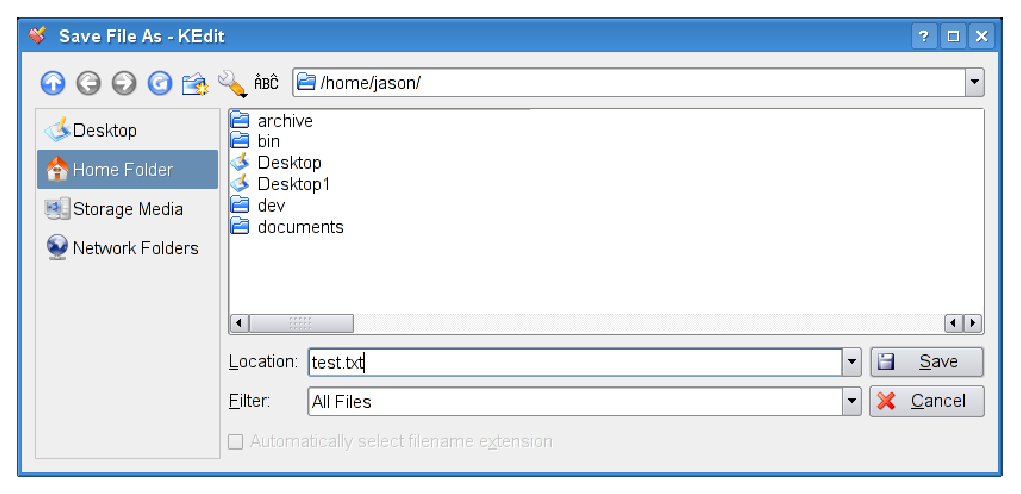
\includegraphics[width=65mm]{eps/figure19.eps}
\end{center}
\caption{The save dialog from the KEdit Text Editor.}\label{fig19}
\end{figure}

Open the Python console again, and try the following:

\begin{listing}
\begin{verbatim}
>>> f = open('Desktop/test.txt')
>>> print(f.read())
\end{verbatim}
\end{listing}

\end{LINUX}

So what does that little bit of code do?  The first line calls the function \code{file}, passing the name of the file you just created, as a parameter.  The function returns a special type of value (called an object) which represents that file.  It's not the file itself; rather it's a bit like a big finger pointing at the file going ``HERE IT IS!!!!''  The file object is stored in the variable \code{f}.
\par
The next line calls a special function (\code{read}) on the file object, to read in the contents of the file, and print the result to the console.  Because the variable \code{f} contains an object, this means we need to call the read function using the dot symbol (.).

\fbox{\colorbox{PaleBlue}{\parbox{.75\linewidth} {
\par
Appendix~\ref{app:builtinfunctions} (at the back of this book) has more information about the functions that are built into Python.
\par
}}}

\section{Modules}\index{modules}

We've actually seen a couple of different ways to reuse code already. One is a standard function, which we can create ourselves, or use the functions built into Python (like \code{range} and \code{file} and \code{int} and \code{str}). Another is a special kind of function on objects---which we can call using the dot symbol---and the next are modules; which are a way of grouping lots of functions and objects together in useful ways. An example of this is the module `time'\index{modules!time}:

\begin{listing}
\begin{verbatim}
>>> import time
\end{verbatim}
\end{listing}

The import command is used to tell Python we want to access a module.  In the above example, we're saying we want to use the `time' module. We can then call functions and objects that are available in this module, using the dot symbol yet again:

\begin{listingignore}
\begin{verbatim}
>>> print(time.localtime())
(2006, 11, 10, 23, 49, 1, 4, 314, 1)
\end{verbatim}
\end{listingignore}

localtime\index{modules!time!localtime} is a function \emph{inside} the module time, that returns the current date and time, broken up into individual parts---year, month, day, hour, minute, second, day of the week, day of the year, and whether or not it's daylight savings (1 if it is, 0 if it isn't).  The individual parts are stored in a tuple (see \emph{Tuples and Lists} on page~\pageref{tuplesandlists}.  You can use another function in the time module to convert the datetime returned by localtime, into something a bit more understandable:

\begin{listingignore}
\begin{verbatim}
>>> t = time.localtime()
>>> print(time.asctime(t))
Sat Nov 18 22:37:15 2006
\end{verbatim}
\end{listingignore}

\noindent
We can do that all in a single line if we wanted to:

\begin{listingignore}
\begin{verbatim}
>>> print(time.asctime(time.localtime()))
Sat Nov 18 22:37:15 2006
\end{verbatim}
\end{listingignore}

Suppose you want to ask for someone to enter a value. You can do this using a \code{print} statement and the module `\code{sys}'\index{modules!sys}---imported the same way we imported the \code{time} module:

\begin{listing}
\begin{verbatim}
import sys
\end{verbatim}
\end{listing}

Inside the sys module is an object called `stdin'\index{modules!sys!stdin} (short for standard input).  stdin has a rather useful method (or function) called \code{readline}---which is used to read a line of text someone types on the keyboard (up until the point when they press the Enter key).  You can test \code{readline}, by entering the following command in the Python console:

\begin{listing}
\begin{verbatim}
>>> print(sys.stdin.readline())
\end{verbatim}
\end{listing}

If you then type some words, and press the Enter key, what you've typed will be printed to the console. Think back, for a moment, to the code we wrote earlier, using an if-statement:

\begin{listing}
\begin{verbatim}
if age >= 10 and age <= 13:
    print('you are %s' % age)
else:
    print('huh?')
\end{verbatim}
\end{listing}

Rather than creating the variable \code{age} beforehand, we can now ask someone to enter the value instead.  How about first turning the code into a function$\ldots$

\begin{listing}
\begin{verbatim}
>>> def your_age(age):
...     if age >= 10 and age <= 13:
...         print('you are %s' % age)
...     else:
...         print('huh?')
... 
\end{verbatim}
\end{listing}

Which can be called, by passing a number as the parameter value.  We'll test that it works properly, first:

\begin{listing}
\begin{verbatim}
>>> your_age(9)
huh?
>>> your_age(10)
you are 10
\end{verbatim}
\end{listing}

Now we know there are no problems with our function, we can change the function to ask for a person's age instead:

\begin{listing}
\begin{verbatim}
>>> def your_age():
...     print('Please enter your age')
...     age = int(sys.stdin.readline())
...     if age >= 10 and age <= 13:
...         print('you are %s' % age)
...     else:
...         print('huh?')
... 
\end{verbatim}
\end{listing}

Because \code{readline()} returns what a person typed as text (in other words, a string), we need to use the function \code{int} to convert it to a number (this so it will work correctly in the if-statement---check \emph{What's the difference} on page~\pageref{whatsthedifference} for more information about this).  To try it for yourself, call the your\_age function without any parameters, then type some text when `Please enter your age' appears:

\begin{listingignore}
\begin{verbatim}
>>> your_age()
Please enter your age
10
you are 10
>>> your_age()
Please enter your age
15
huh?
\end{verbatim}
\end{listingignore}

\noindent
\emph{The important thing to note here is that even though you're typing in a number (in the above case 10 or 15), readline always returns a string.}

\fbox{\colorbox{PaleBlue}{\parbox{.75\linewidth} {
\code{sys} and \code{time} are just two of the many modules that are included with Python.  For more information on some (but not all) Python modules, see Appendix~\ref{app:afewpythonmodules}.
}}}

\section{Things to try}

\emph{In this chapter we saw how to do recycling in Python; through the use of functions and modules.  We saw a little bit about the `scope' of variable, how variables outside of functions can be `seen' inside, whereas variables inside cannot be seen outside, and learned how to create our own functions using \code{def}}

\subsection*{Exercise 1}
In exercise 2 in Chapter~\ref{ch:againandagain}, we created a for-loop to work out the interest we might earn from \$100 over a period of 10 years.  That for-loop could easily be turned into a function.  Try creating a function which takes a starting amount, and a rate of interest.  You could call the function using code like:

\begin{listing}
\begin{verbatim}
calculate_interest(100, 0.03)
\end{verbatim}
\end{listing}

\subsection*{Exercise 2}
Take the function you've just created, and make it calculate interest for different periods---such as 5 years or 15 years.  Perhaps you could call it using code like:

\begin{listing}
\begin{verbatim}
calculate_interest(100, 0.03, 5)
\end{verbatim}
\end{listing}

\subsection*{Exercise 3}
Perhaps rather than a simple function, where we pass in the values as parameters, we can make a mini-program which asks someone for the values (using the \code{sys.stdin.readline()} function).  In this case, we'll call the function without any parameters at all:

\begin{listing}
\begin{verbatim}
calculate_interest()
\end{verbatim}
\end{listing}

\noindent
To create this mini-program requires a function that we haven't talked about yet: \code{float}. The \code{float} function is a bit like the \code{int} function, except it converts strings into what is called floating point numbers (which we discussed briefly in Chapter~\ref{ch:8multipliedby3.57}).  Floating point numbers are numbers with a decimal place (.), such as 20.3 or 2541.933.

\newpage
